%----------------------------------------------------------------------------   
\chapter{Használt eszközök bemutatása}
%---------------------------------------------------------------------------- 

\section{Kubernetes}

A Kubernetes egy nyílt forráskódú konténer kezelő platform, amivel automatizálni
lehet a legtöbb feladatot, ami a fejlesztés, karbantartás vagy skálázással 
kapcsolatos. A Google fejlesztette eredetileg, de jelenleg a Cloud Native
Computing Foundation - CNCF vette át a karbantartását. 

Kubernetes fürtöt létrehozhatunk lokálisan a saját szerveren is vagy felhőben,
ami lehet publikus, privát vagy hibrid hozzáférésű. Viszont azt figyelembe 
kell venni, hogy egy Kubernetes fürtöt nem egyszerű kiépíteni lokálisan, 
szóval ha nem szükséges, akkor lehet használni felhőszolgáltatók Kubernetes 
motorjai, mint az Amazon AKS, Linode LKE vagy a Google GKE szolgáltatása.
Ilyenkor egy teljes fürtöt, ami az általunk beállított paramétereket használja.

\subsection{Felépítése}

\begin{figure}[!ht]
	\centering
	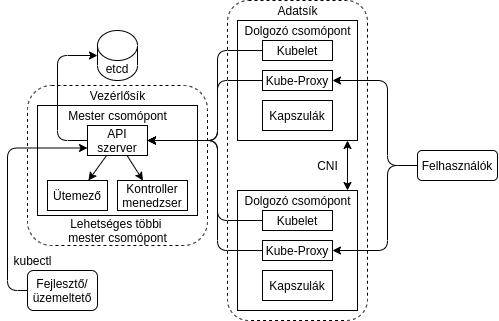
\includegraphics[width=1\textwidth, keepaspectratio]{figures/k8s_architecture.png}
	\caption{Kubernetes fürt felépítése}
	\label{fig:HVSpaces}
\end{figure}

Egy Kubernetes fürt kettő részből áll egy vezérlő- és egy adatsíkból, ahol a 
vezérlősíkban szereplő mester csomópontok tudják vezérleni az adatsíkban 
lévő dolgozó csomópontokat és a fejlesztők vagy üzemeltetők a mester által
hirdetett API-n keresztül képesek parancsokat kiadni. Míg a dolgozó 
csomópontokon futó alkalmazáshoz a felhasználók csak az általuk hirdetett 
Kube-Proxy segítségével tudnak hozzáférni. 

A kapcsolat mester és dolgozó között az API szerver és a Kubelet kommunikációján
alapul. Ha a fejlesztő szeretne egy új alkalmazást telepíteni a fürtön, akkor
szól az API szervernek, ami majd kiadja a megfelelő parancsokat a Kubelet-nek 
és majd az fogja a konténereket létrehozni. Amiről az API szervert értesítve 
tudja meg a fejlesztő, hogy amit csinált az létrejött.

\subsubsection{Vezérlősík}

A mester csomópont mindig a fő vezérlő egysége a fürtnek, mivel kezeli a 
munkafolyamatokat és irányítja a kommunikációt fürtön belül. A 2.1-s ábrán
látható vezérlősík tartalmazhat  több mester csomópontot is a felsorolt 
komponensekkel, amivel lehet biztosítani a fejlesztők számára a folytonos 
elérést. A mester csomópont részei: 

\begin{itemize}
	\item \textbf{etcd}: Egy állandó kulcs-érték alapú adatbázis, ami tárolja 
	a fürt konfigurációs beállításait és a fürt állapotát. Fontos az a rész, 
	hogy ez egy állandó adatbázis, mivel ez a csomóponton fut és nem egy 
	kapszulában.   
	\item \textbf{API szerver}: Egy REST API szerver, ami hozzáférést biztosít
	a fürthöz a fürtön belül és azon kívül is. Egyszerű HTTP üzenetekbe ágyazott
	JSON konfigurációkkal lehet beállítani, hogy mit csináljon a fürtben. De 
	a dolgozó csomópontok is ezen keresztül küldenek frissítést az etcd-be. 
	\item \textbf{Ütemező}: Ez a komponens dönti el, hogy egy új kapszula melyik
	dolgozó csomóponton legyen létrehozva aszerint, hogy van-e megfelelő erőforrás
	az adott csomópontot megvalósító szerveren.
	\item \textbf{Kontroller menedzser}: Egy olyan állandóan futó folyamat ellenőri,
	hogy a kapszulákból bizonyos esetekben újrainduljanak vagy hogy egy ismétlődő 
	munkafolyamot időnénként lefusson helyesen. Ezt az API szerverrel kommunikálva
	képes megvalósítani. 
\end{itemize}

Mint ahogy az ábrán is látszik a fejlesztő vagy üzemeltető alapvetően a \textbf{kubectl}
nevezetű eszközzel képesek kommunikálni az API szerverrel. Ez az eszköz lényegében
megvalósítja a teljese HTTP kommunikációt az API szerverrel szóval sokkal könnyebben 
lehet vele lekérdezni információkat vagy új erőforrásokat létrehozni. 

\subsubsection{Adatsík}

Az adatsíkon futnak az úgynevezett dolgozók, amik igazából különálló szerverek,
amik rendelkeznek a 2.1-s ábrán szereplő komponensekkel és képesek futtatni 
valamilyen konténer kezelő alakalmázást, mint például a Docker. Ami régebben az 
alapértelmezett konténer kezelője volt a Kubernetes-nek, de 2021-ben már nem 
követeli meg és bármilyen másik konténer kezelőt is be lehet állítani alapértelmezettnek.

A fontosabb elemei az adatsíknak:

\begin{itemize}
	\item \textbf{Kubelet}: Felelős az egyes csomópontok futási állapotáért biztosítva, 
	hogy a csomóponton lévő összes konténer egészséges legyen. Gondoskodik az alkalmazás
	konténereinek indításáról, leállításáról és karbantartásáról, amelyek kapszulákba 
	vannak rendezve a vezérlősík utasítása szerint
	\item \textbf{Kube-Proxy}: Egy proxy és terheléselosztó megvalósítása, ami biztosítja
	a szolgáltatás elérhetőségét más hálózatok számára. Így a feladat az, hogy a beérkező
	forgalmat a megfelelő konténerekhez irányítsa a bejövő kérelem IP címe és 
	portja alapján. 
	\item \textbf{Kapszulák}: A legkisebb menedzselhető egységek amiket lehet telepíteni
	Kubernetes alatt. Egy kapszula több konténernek a csoportja, amik osztoznak a tárolási
	és hálózati erőforrásokon és specifikálja, hogy a konténerek hogyan fussanak. 
	\item \textbf{CNI}: A hálózati interfészeit lehet konfigurálni a konténereknek.
\end{itemize}

\subsection{Erőforrások}

A fentebb leírt architektúra csak az alapjai a Kubernetesnek, viszont ezen kívül
még rengeteg olyan erőforrással is rendelkezik, amik lehetővé teszik a konténerek
menedzselésének egy új szintjét.

A következőkben leírom, hogy a projekt szempontjából mely erőforrások lesznek még
lényegesebbek. 

\begin{itemize}
	\item \textbf{Replikációs vezérlő}: Biztosítja, hogy egy meghatározott számú 
	kapszula replika fusson egyszerre, amivel biztosítja az alkalmazás magas szintű
	elérhetőségét. Ami azt eredményezi, ha túl sok kapszula fut, de nem kellene nekik,
	akkor törli azokat vagy, ha túl kevés, akkor újakat hoz létre. Mindazonáltal, 
	ha egy kapszula maga vagy az egyik konténere hibát eredményez, akkor újraindítja
	a benne lévő konténer vagy a teljes kapszulát. 
	\item \textbf{Telepítő (Deployment}): Leírja egy elvárt állapotot, ami alapján a
	replikációs vezérlő tudja, hogy milyen specifikáció szerint kell az új kapszulákat
	létrehozni vagy a kapszulák számát. 
	\item \textbf{DaemonSet}: Biztosítja, hogy az összes vagy néhány csomópont 
	futtassa egy meghatározott kapszula másolatát. Így, ha egy új dolgozó csomópont 
	csatlakozik a fürthöz, akkor ez a kapszula automatikusan megjelenik rajta. Tipikusan
	valamilyen tárolási vagy monitorozási feladatot ellátó kapszulát szokás ilyen
	módon létrehozni, de a későbbiekben látni fogjuk, hogy az l7mp ugyan ezzel a 
	módszerrel hozza létre a bejárati pontokat a csomópontokon.
	\item \textbf{DNS}: Tárolja a fürtben szereplő minden kapszula és szolgáltatás
	IP címét illetve a hozzájuk kapcsolódó tartomány nevüket is.  
	\item \textbf{Szolgáltatás}: Egy absztrakt módja az alkalmazást futtató kapszulák
	kiexponálásának a hálózaton keresztül. Mivel a kapszulák halandóak így nem mindig
	ugyanazon a címen lesznek elérhetőek a rajtuk futtatott alkalmazások. A megoldás
	erre, ha egy címke alapján hozzárendeljük őket egy szolgáltatáshoz, ami mindig 
	elérhető lesz ugyanazon a címen és képes elosztani a forgalmat több kapszula között.
	A forgalomirányítást a szolgáltatások a Kubernetes DNS szolgáltatása miatt tudják 
	megvalósítani.  
	\item \textbf{Bejárat (Ingress gateway)}: Egy olyan API objektum, ami kezeli a 
	külső hozzáférést különböző szolgáltatásokhoz a fürtön belül. Így a bejövő forgalmat
	könnyen lehet szűrni illetve típusától tartalmától függően más és más szolgáltatásokhoz
	lehet irányítani. 
	\item \textbf{Egyéni erőforrás definíció (Custorm Resource Definition)}: A 
	Kubernetes API egy olyan kiterjesztése melynek során új fajta erőforrás definíciókat
	lehet definiálni. 
	\item \textbf{Pótkocsi (Sidecar)}: Mivel egy kapszula több konténert is tartalmazhat
	és ezek a konténerek megosztják a hálózatukat így létre lehet hozni egy olyan konténert
	ami csak a hálózati forgalom kezelésével foglalkozik. Így könnyen lehet szűrni, hogy
	milyen forgalom juthat csak el az alkalmazást futtató konténerhez. 
	\item \textbf{RBAC (Role-based access controll)}: Ha több fejlesztő vagy üzemeltető
	fér hozzá az API szerverhez, akkor egyénenként meglehet mondani, hogy kinek milyen 
	művelet végrehajtására van joga. Így például korlátozható, hogy ki képes új
	erőforrásokat létrehozni. De ez nem csak igazi felhasználókra vonatkozik, hanem
	kapszulákra is. Ezáltal lehet olyan kapszulákat létrehozni, amik képesek a fürtön
	belül kommunikálni az API szerverrel és erőforrásokat kezelni.  
	\item \textbf{Operátor}: Olyan bővítések, amikkel egyéni erőforrások menedzselése
	valósítható meg. De emellett különböző eseményeknél lehet bizonyos folyamatokat 
	elindítani. Példának okáért, ha egy kapszula létrejön, akkor beállíthatjuk, hogy
	rendelkezzen mindig egy adott címkével.
	\item \textbf{Szolgáltatás háló (Service Mesh)}: Meghatározza, hogy a fürt 
	különböző részei hogyan kommunikáljanak egymással. Ezt általában a pótkocsikkal és 
	egy operátorral valósítják meg. A pótkocsik fognak rendelkezni azokkal a beállításokkal,
	hogy milyen a mellettük futó konténer milyen forgalmat fogadhat és az operátor 
	fog arról gondoskodni, hogy a résztvevő kapszulák pótkocsijai mindig a megfelelő
	beállításokkal jöjjenek létre.
\end{itemize}

\section{L7mp}

Az l7mp egy kísérleti alkalmazásréteg és több protokollt támogató szolgáltatás- 
proxy és háló keretrendszer. A hangsúly a több protokoll támogatásán van, amely
lehetővé teszi, hogy sok szállítási és alkalmazásréteg béli protokollt 
natívan támogasson és ne csak a szokásos TCP/HTTP protokollokat. Lehetővé teszik 
emellett még a protokollok közötti konvertálást is így könnyen lehet alkalmazási
rétegű protokollokat konvertálni szállításiba és vissza is.

Az l7mp, mint a Kubernetes áll egy vezérlő- és adatsíkból. Ahol az adatsíkot 
az l7mp proxy valósítja meg. Míg a vezérlőt egy operátor, ami képes kezelni 
az l7mp proxy példányokat. 

Ha egy másik szoftverhez kellene hasonlítanom az l7mp-t akkor az az Istio 
lenne, ami egy népszerű szolgáltatás háló az Envoy-l kombinálva. Azért 
hasonlítanám leginkább ehhez, mert az l7mp proxy nagyon hasonlóan működik az
Envoy-hoz képest. Szóval, aki ezeket a rendszereket jobban ismeri az 
könnyen eligazodik az l7mp keretrendszeren is.\\

Szeretném megemlíteni, hogy Dr. Rétvári Gábor Ferenc vezetésével a nyári
gyakorlati időm alatt és jelenlegi munkámként ennek a szoftvernek a tesztelésével 
illetve fejlesztésével foglalkozom, így viszonylag közel áll hozzám a használata.
Ez azért fontos a szakdolgozat szempontjából, mert jelenleg csak a felhasználói névtérben
képes működni, ami okozhat teljesítménybeli problémákat, amik a későbbiekben 
esetlegesen javítva lesznek és akkor már jobb eredményeket lehet generálni. 

\subsection{L7mp, mint proxy}

Egy olyan programozható proxy, ami nagyon hasonlóan működik, mint az Envoy, ami 
egy széleskörűen használt leginkább alkalmazási réteget támogató proxy. A különbség
az l7mp és az Envoy között, hogy az l7mp a szállítási réteg protokolljait 
támogatja jobban. Emellett tetszőleges számú végpontot tud egymással összekötni, 
amik között könnyen lehet egyik protokollból a másikba váltani. 

A proxy egy magas szintű keretrendszerben íródott, ezért nagyon egyszerűen 
lehet új funkciókkal bővíteni. Ez a keretrendszer a Node.js, ami egy JavaScript
futtató környezet a Google Chrome V8-s JavaScript motorjára építve. Ez szerencsés 
választás a már említett egyszerű bővíthetőség miatt, de  amiatt is, hogy
könnyen lehet vele aszinkron módon programozni. Így nincsenek blokkoló műveletek,
amiket külön szálon kellene futtatni. De behozza azt a hátrányt is, hogy a 
JavaScript miatt lassabb az l7mp, mint az Envoy, ami C++-ban van írva. 

A lassúság kiküszöbölésére jelenleg vannak munkálatok, amik elsősorban azt 
célozzák meg hogy a csomagok feldolgozása nem a felhasználói névtérben kerüljenek
végrehajtásra, hanem kernel szinten. Így a csomagoknak nem kell fájlleírókon 
keresztül eljutnia az l7mp-hez, hanem az l7mp konfigurálása folyamán lehetne
olyan iptables szabályokat létrehozni, amik megoldják a csomagok továbbítását
anélkül, hogy írni vagy olvasni kellene a fajleírókat. Az iptables egy olyan 
kernel szintű program, amely lehetővé teszi a csomagok feldolgozását és továbbítását
a kernelben. \\

Az l7mp, mint önálló proxy használható szimplán Node-l, mivel elérhető az NPM
csomagkezelőben és emellett Docker képfájllal is rendelkezik. 

\subsubsection{Felépítése}

Mivel az l7mp tervezése során az Envoy volt a minta, így főbb elemei között szerepelnek
ugyanolyan vagy hasonló elemek. A legfontosabb építőkockái az l7mp-nek 
felsorolásra és kifejtésre kerülnek alább: 

\begin{itemize}
	\item \textbf{Munkamenet (Session)}: Munkameneteket nem lehet manuálisan létrehozni,
	mivel ezek akkor generálódnak, amikor egy figyelő forgalmat kap és azt 
	továbbítja valamerre. Egy munkamenet információkat tartalmaz a csomagok típusáról,
	forrás címéről és céljáról. Emellett a munkamenet objektum felelős azért is, hogy a
	a benne lévő objektumok tudják, hogy a hozzájuk beérkező csomagokat fel kell dolgozniuk. 
	\item \textbf{Figyelő (Listener)}: Definiálni lehet vele egy cím és port párost, hogy
	adott protokollal rendelkező csomagokra figyeljen és dolgozza fel őket. A feldolgozás
	alatt azt a folyamatot kell érteni, hogy meghatározza mely fürthöz kerüljön a csomag,
	szűri hogy a bejövő csomagok fejlécében szerepel-e valamilyen meghatározott érték és 
	ezeket a fejléc mezőket módosítani is lehet. Ez különösen hasznos funkció, akkor 
	amikor JSONSocket vagy WebSocket forgalmat kell kezelni. 
	\item \textbf{Fürt (Cluster)}: A végpontok egy gyűjteménye, ami képes forgalmat elosztani
	közöttük. Az elosztás történhet nagyon egyszerűen, amikor mindig egy lista élén álló
	végpont kapja a forgalmat, de történhet HashRing módszerrel is. Amikor egy kulcs szerint
	történik a végpont kiválasztása. Ez egy hasznos funkció, mivel így fix kulcs mellett,
	minden csomag ugyanahhoz végponthoz fog kerülni. 
	\item \textbf{Végpont (Endpoint)}: A csomag végállomása, ami lehet a már a csomagokat
	feldolgozó alkalmazás vagy egy másik figyelő is. Így egész komplex folyamatokat 
	lehet kiépíteni, ha szükség van rá. 
	\item \textbf{Szabály (Rule)}: Szabályokat a figyelőkben lehet létrehozni, amikkel
	belehet állítani, hogy mi legyen a célja a beérkező csomagoknak vagy meglehet vele azt
	is határozni, hogy a fejléc mely paraméterét mire módosítsa. 
	\item \textbf{Útvonal (Route)}: Meghatározza a célt, ami általában egy fürt. Az 
	útvonalak mindig a szabályokon belül vannak, hiszen a szabályok határozzák meg a célt.
	De ezen felül még be lehet azt is állítani, hogy a bejövő csomagok milyen útvonalon 
	jussanak el a fürtig és milyen vissza. Így a bejövő és kimenő forgalmat teljesen 
	más útvonalon lehet irányítani.
\end{itemize}

Ezekkel az elemekkel és az egyszerűségük miatt rendkívül egyszerűen lehet konfigurálni
az l7mp-t. 

\subsubsection{Programozása}

Az l7mp programozása történhet konfigurációs fájlból és REST API hívásokon keresztül
egyaránt. Viszont az l7mp indításához szükség van egy alapkonfigurációra, mivel
anélkül nem fog létrejönni a kontroller figyelő, ami biztosítja az API 
láthatóságát. Az alábbi kódrészleten látható, hogyan lehet egy ilyen induló konfigurációt
létrehozni. 

\begin{lstlisting}
	admin:
      log_level: info
      log_file: stdout
      access_log_path: /tmp/admin_access.log
	listeners:
      - name: controller-listener
		spec: { protocol: HTTP, port: 1234 }
		rules:
		  - action:
			   route:
			     destination:
		           name: l7mp-controller
		           spec: { protocol: L7mpController }
\end{lstlisting}

A konfigurációt részről részre kifejtem. Az első része, az \textit{admin}, ahol
a naplózás szintjét és helyét lehet meghatározni. A következő szintek vannak:
silly, verbose, info, notice, warn, error, silent. Amik ebben a sorrendben
egyre kevesebb információt naplóznak. A silly kiírja a beérkező csomagok tartalmát
is, míg az info már csak munkafolyamat mélységig működik.

Az utána következő részben létre jön a controller-listener, ami helyi hálózaton az 
1234 porton hirdeti a REST API pontot, amin keresztül később új konfigurációkat lehet 
konfigurálni. Ehhez egy olyan protokoll van használva, ami nem egy igazi protokoll
csak ezzel van jelezve, hogy hozza létre API pontot. 

Ez az API megvalósítja a teljes CRUD-t mindent komponensre, amivel tudunk létrehozni, 
olvasni, frissíteni és törölni komponenseket. Minden komponenshez tartozik egy útvonal, 
ami így tevődik össze, ha a fenti példát nézzük: http://127.0.0.1:1234/api/v1/listeners.
Ha erre a címre egy POST üzenetben YAML vagy JSON konfigurációt küldünk, akkor az
létre fog jönni a proxy-n belül. Ami még egy hasznos funkció ebben a megvalósításban
az a rekurzív lekérés, aminek során egy GET üzenettel és az URI paraméterekben a 
\textbf{recursive=true} paraméter beállításával a figyelők esetében részletesen 
kiíratásra kerül minden benne lévő objektum. Az API teljes dokumentációja 
megtalálható a következő oldalon: https://l7mp.io/openapi/. \\

A következőkben látható lesz egy példa, ami pont az API-n keresztüli programozást
hivatott bemutatni. 

\begin{lstlisting}
	curl -iX POST --header 'Content-Type:text/x-yaml' --data-binary @- <<EOF  http://localhost:1234/api/v1/listeners
	listener:
	  spec:
	    protocol: WebSocket
	    port: 2000
	  rules:
	    - action:
	        route:
	          destination:
	            spec:
  	              protocol: UDP
	              port: 3000
	            endpoints:
	              - spec:
	                  address: 127.0.0.1
	EOF
\end{lstlisting}

A fenti hívásban látható, hogy létrehozunk egy figyelőt, ami a 127.0.0.1:2000-s
címen fog WebSocket csomagokat várni, majd azokat UDP-re konvertálva továbbküldeni 
a 127.0.0.1:3000-s címre.

Ezen a példán látszik igazán, hogy milyen egyszerű az l7mp-vel a protokoll konverzió,
mert ilyen rövid beállítással kettő nagyon különböző protokoll között lehet 
átalakítást végezni.

\subsection{L7mp, mint szolgáltatás háló}

Szolgáltatás háló alatt igazából egy olyan operátora kell gondolni, ami a Kubernetes
API-n (Application Programming Interface) keresztül képes L7mp proxy-k halmazát 
kezelni. Ezáltal könnyen tudjuk az L7mp-t, mint ingress gateway használni és 
mint sidecar az alkalmazás kapszulákban.

Ez az operátor három CRD-t használnak a L7mp proxy-k programozására, amik a következők:
\textbf{VirtualService}, \textbf{Target}, \textbf{Rule}. Ezek sorban a következő proxy 
elemeknek felelnek meg: \textbf{Listener}, \textbf{Cluster}, \textbf{Rule}. \\ 

Egy \textbf{VirtualService} az absztrakt megvalósítási egy szerver oldali foglalatnak címnek. 
Ezenfelül egy VirtualService mögött mindig áll egy Kubernetes szolgáltatás, ami 
szolgáltatja a végpontok címét vagy címkéit az elérhetőség miatt.

VirtualService részei: 

\begin{itemize}
	\item Egy szelektor, ami kiválasztja a definiált kapszulákat címkék alapján.
	\item Egy Listener, ami kezeli a beérkező forgalmat. 
	\item (Opcionális) Egy szabálylista, ami tartalmazhat újraírást, érték ellenőrzést
	és meghatározza a célt. 
	\item (Opcionális) További beállítások.  
\end{itemize}

A kliens oldali foglalatot mindig a \textbf{Target} valósítja meg, de beállíthatóak még a 
következő tulajdonságok is: terhelés elosztás, lokális cím lefoglalása, illetve 
meghatározhatnak még végpontot is, amihez a kliensnek csatlakoznia kellene. Ez 
lehet egy másik Target, konkrét cím vagy egy Listener is. Ezenfelül még meglehet 
határozni a bejövő és kimenő forgalom útját is. Így különböző útvonalakat lehet 
könnyen megvalósítani. 

Ha egy Target egyedi névvel rendelkezik, akkor más L7mp erőforrás könnyen 
felhasználhatja a névére való hivatkozással. Ez mind a három CRD-re igaz, de ha
nem határozunk meg egy konkrét nevet, akkor a rendszer automatikusan generál 
egyet minden erőforrásnak. 

%--------------
% PLACE OF RULE
%--------------